%!TEX root = ../../main.tex

\graphicspath{{../../figures/appendix/}}

\chapter{Pattern classification}
\label{ch:cell_pattern_classification}

\newpage

\section{Supervised and unsupervised analyses}
\label{sec:consistency_analysis}

To investigate the agreement between supervised and unsupervised analysis I try to interpret the different regions of the \ac{t-SNE} plot from~\cite{CHOUAIB_2020}.
With the trained classifiers, I compute the probability for each cell to be in a particular pattern and plot these probabilities on top of the \ac{t-SNE}.
In Figure~\ref{fig:tsne_proba_gene} we can observe that cells with high probability of a given pattern concentrated in the same area of the \ac{t-SNE} plot.
Therefore, the embedding appears consistent and a direct interpretation of the point cloud regions seems possible.
In addition, we can notice that the assignments of the classifiers are consistent with the manual annotations illustrated in Figure~\ref{fig:tsne_annotation_racha}.

\begin{figure}[h]
	\centering
	\minipage{0.2\textwidth}
		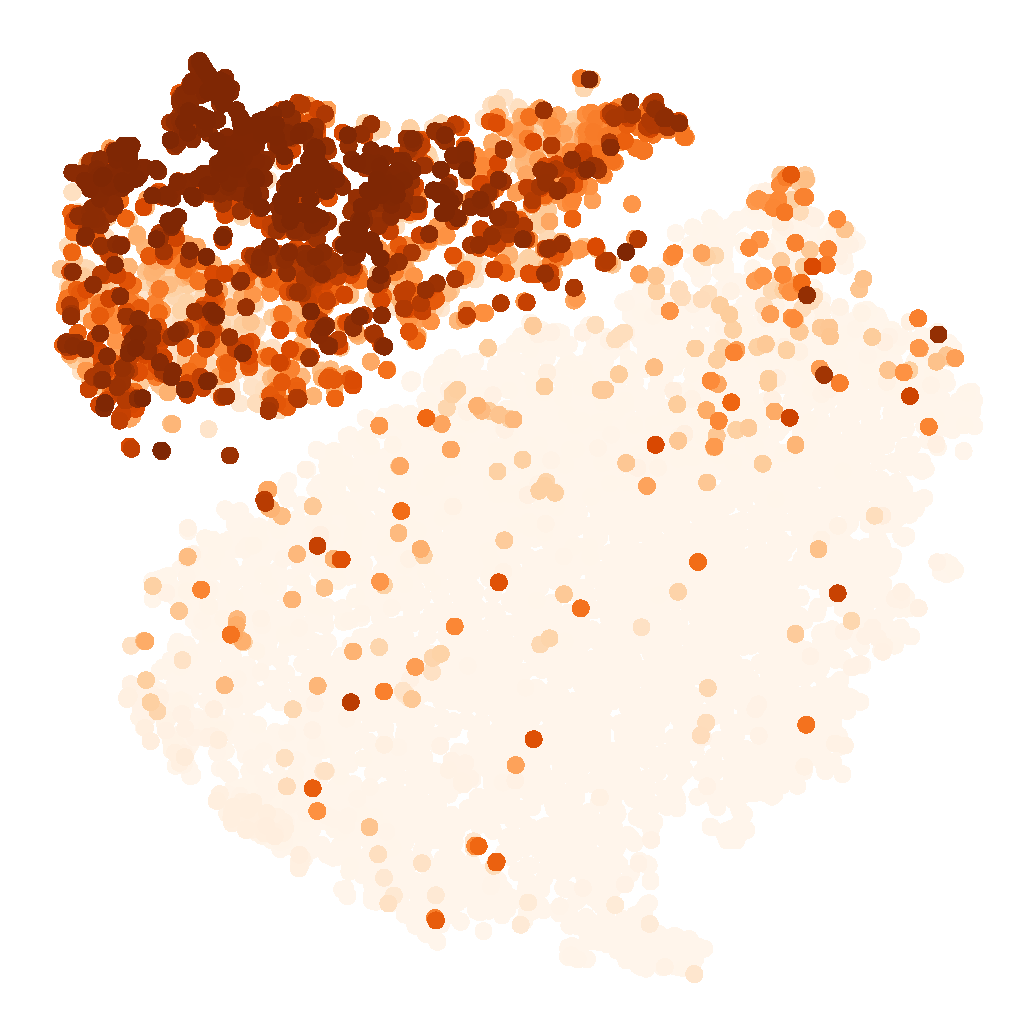
\includegraphics[width=\linewidth]{figures/appendix/tsne_probability_nocolorbar_foci}
		\subcaption{Foci}
		\vfill
		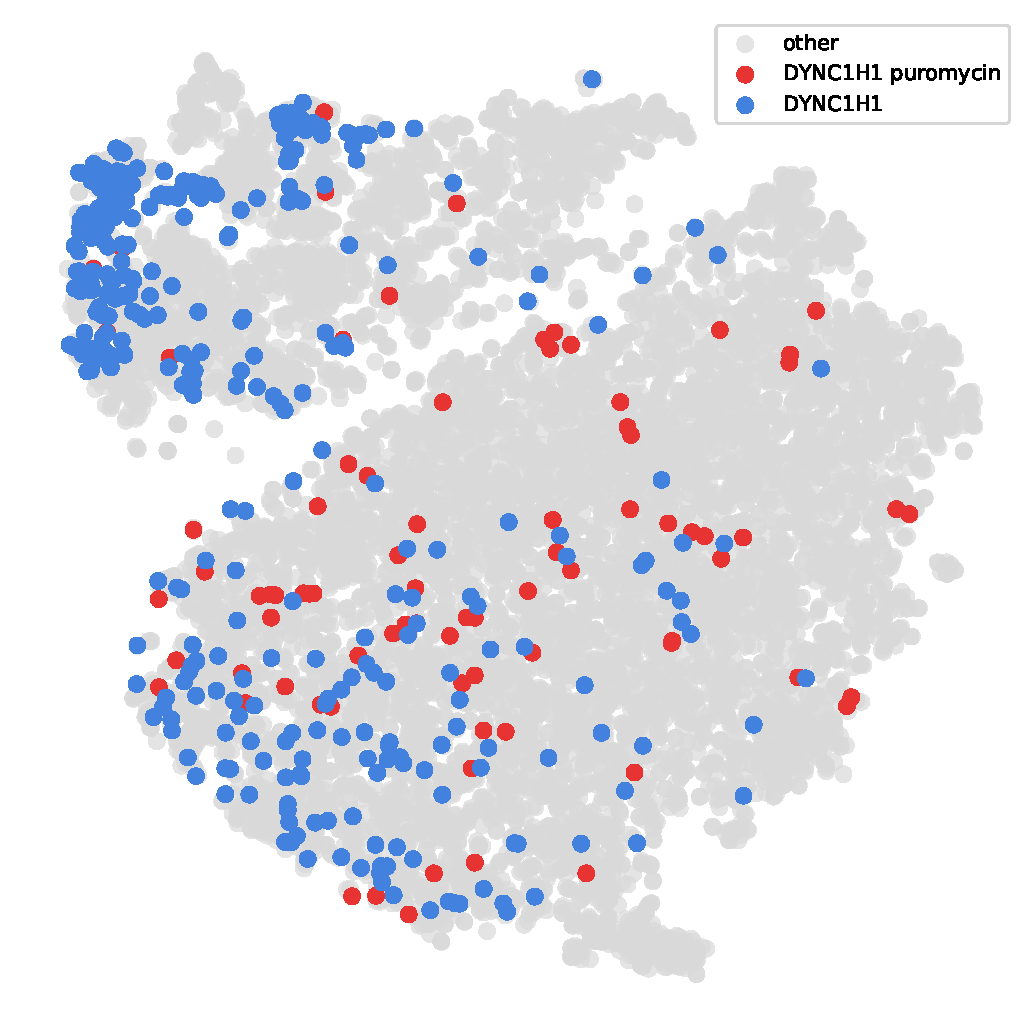
\includegraphics[width=\linewidth]{figures/appendix/tsne_foci_DYNC1H1}
		\subcaption{DYNC1H1}
	\endminipage\hfill
	\minipage{0.2\textwidth}
		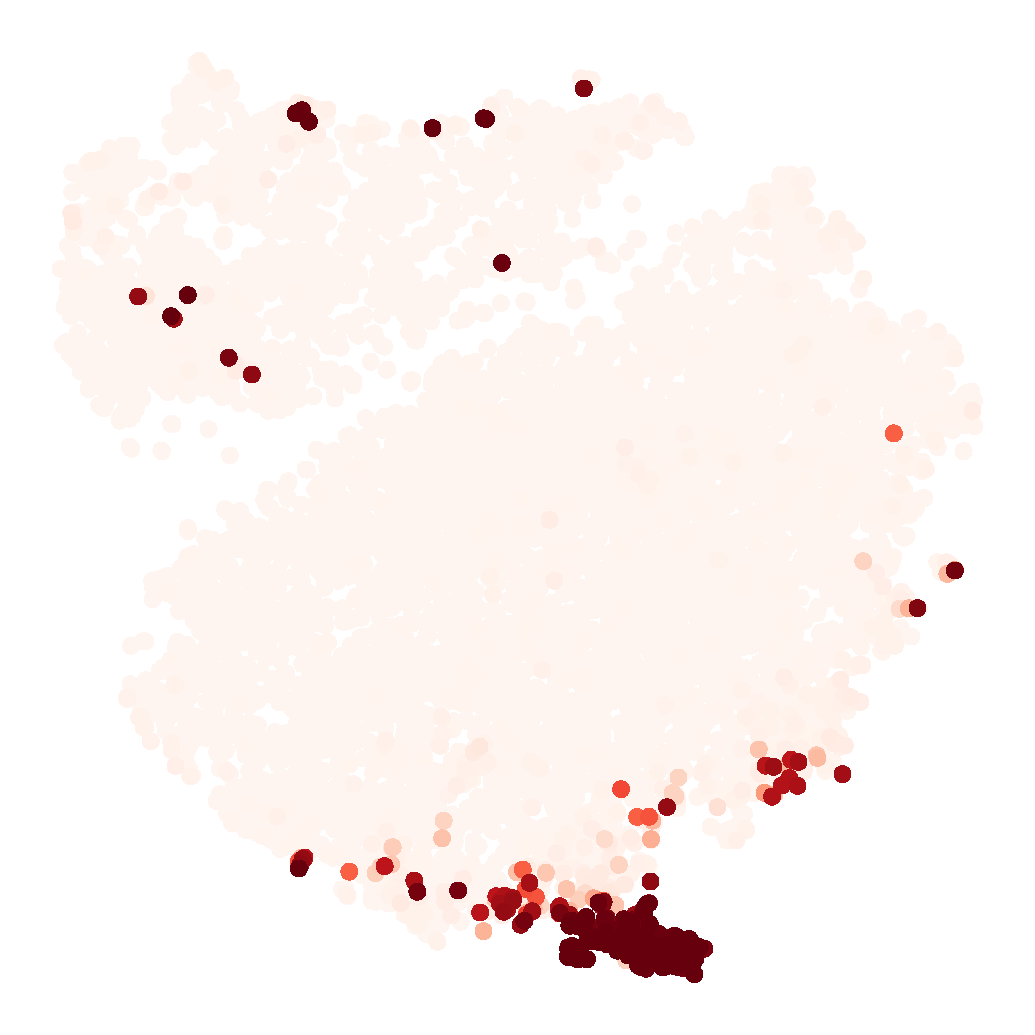
\includegraphics[width=\linewidth]{figures/appendix/tsne_probability_nocolorbar_intranuclear}
		\subcaption{Intranuclear}
		\vfill
		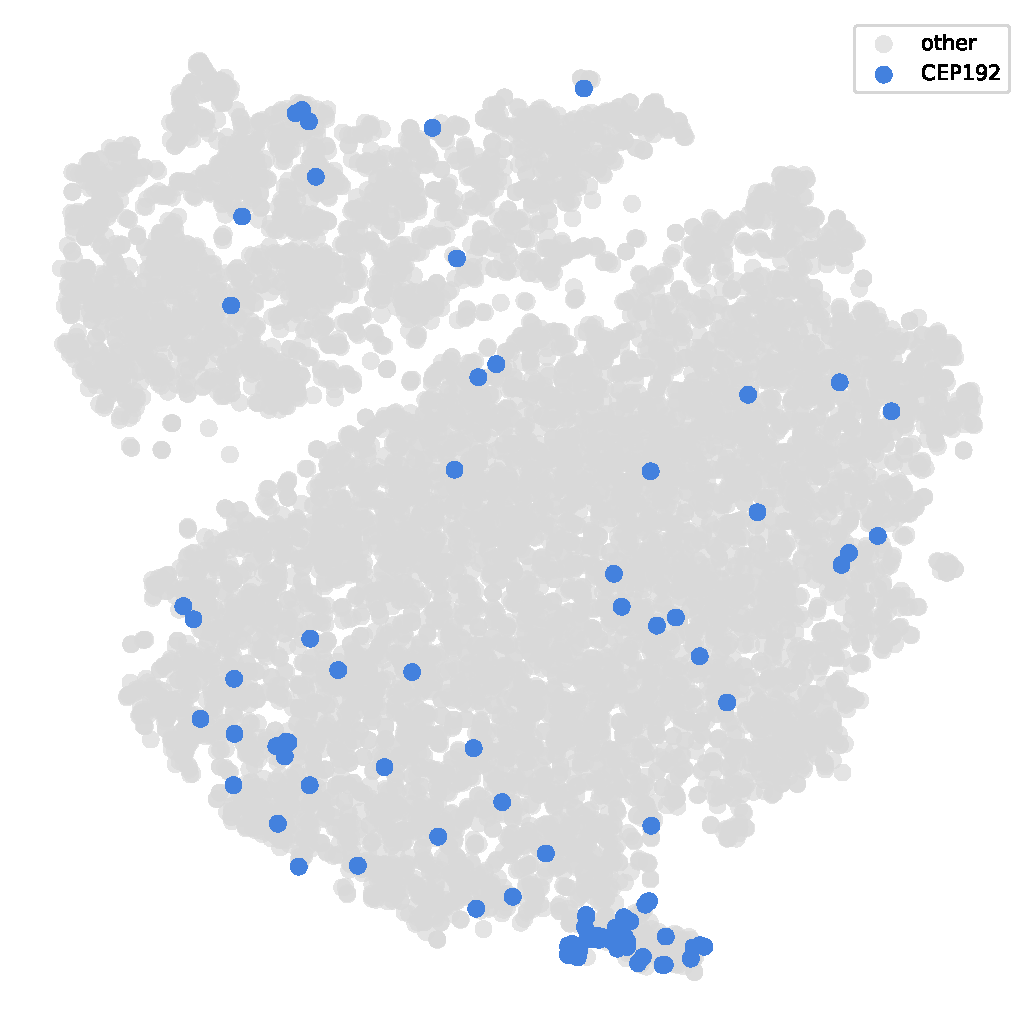
\includegraphics[width=\linewidth]{figures/appendix/tsne_intranuclear_CEP192}
		\subcaption{CEP192}
	\endminipage\hfill
	\minipage{0.2\textwidth}
		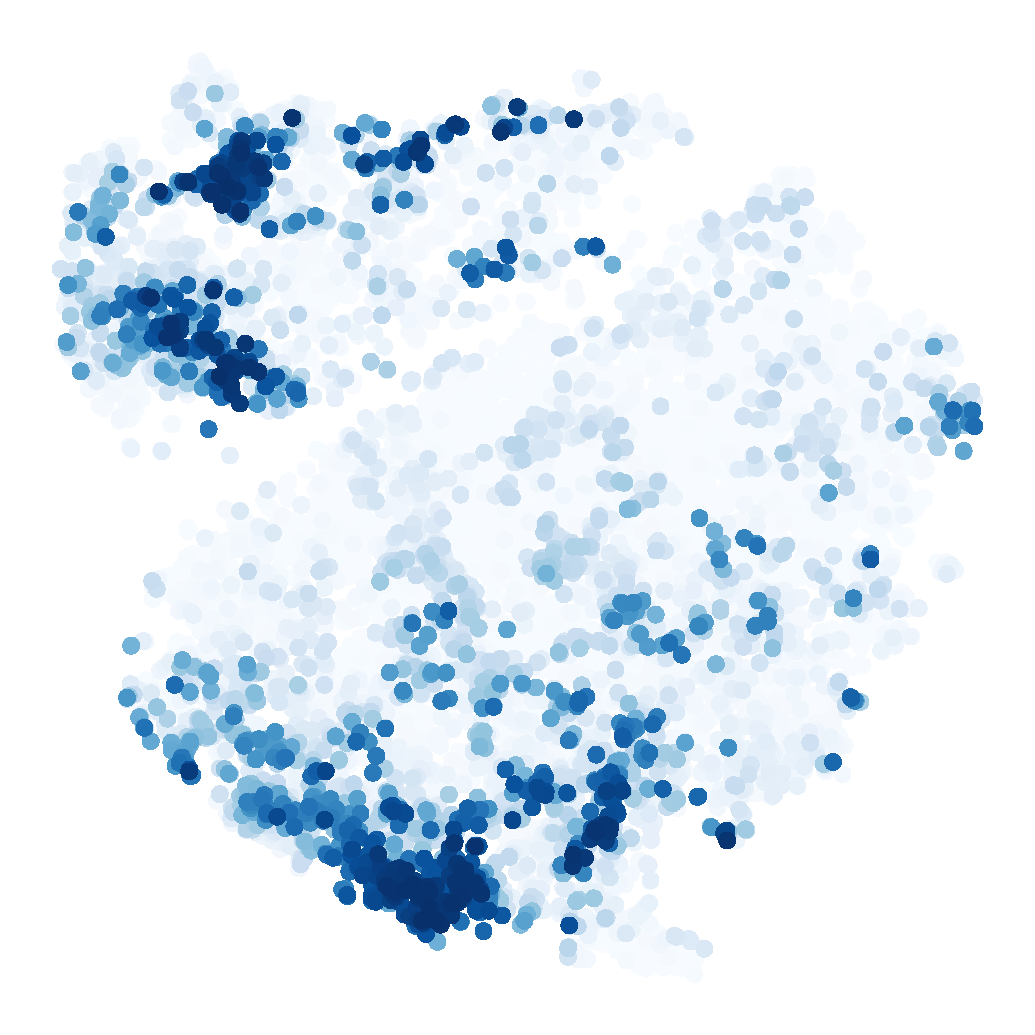
\includegraphics[width=\linewidth]{figures/appendix/tsne_probability_nocolorbar_nuclear}
		\subcaption{Nuclear edge}
		\vfill
		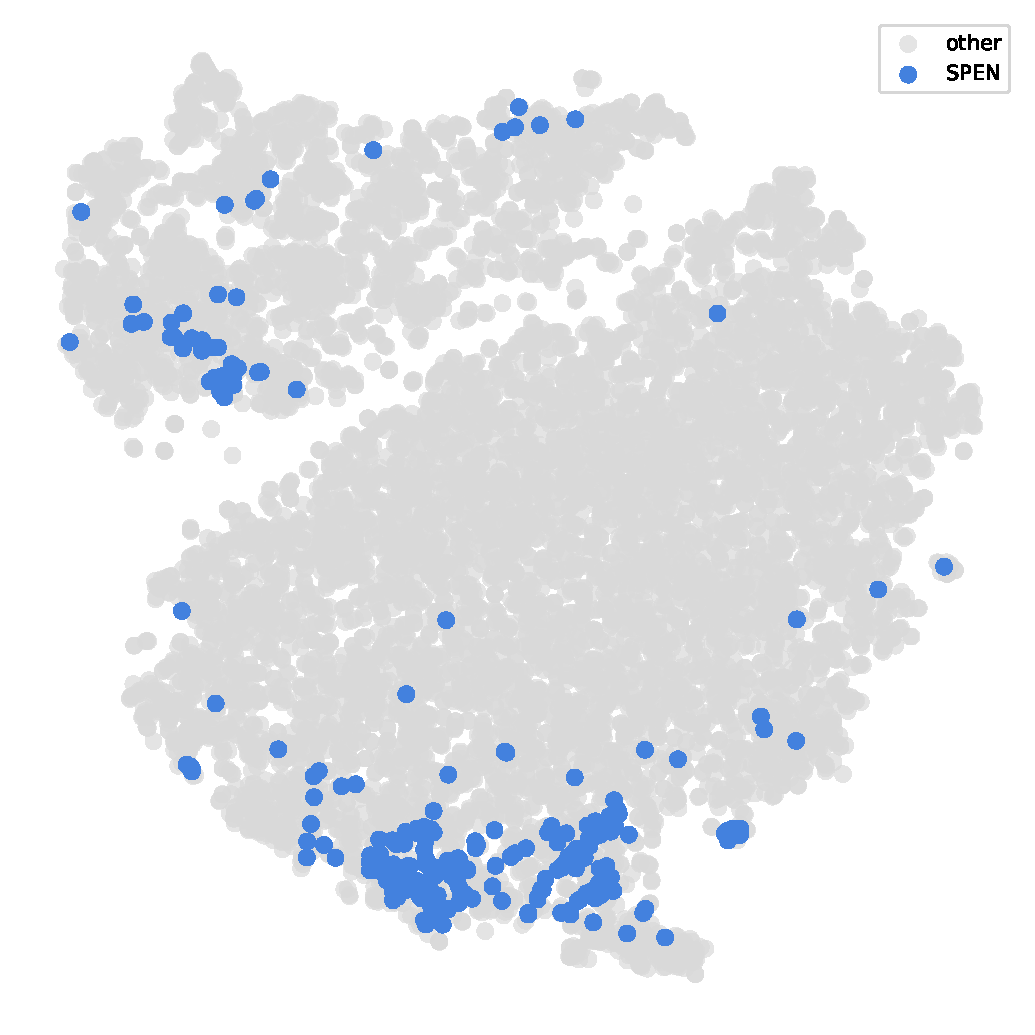
\includegraphics[width=\linewidth]{figures/appendix/tsne_nuclear_SPEN}
		\subcaption{SPEN}
	\endminipage\hfill
	\minipage{0.2\textwidth}
		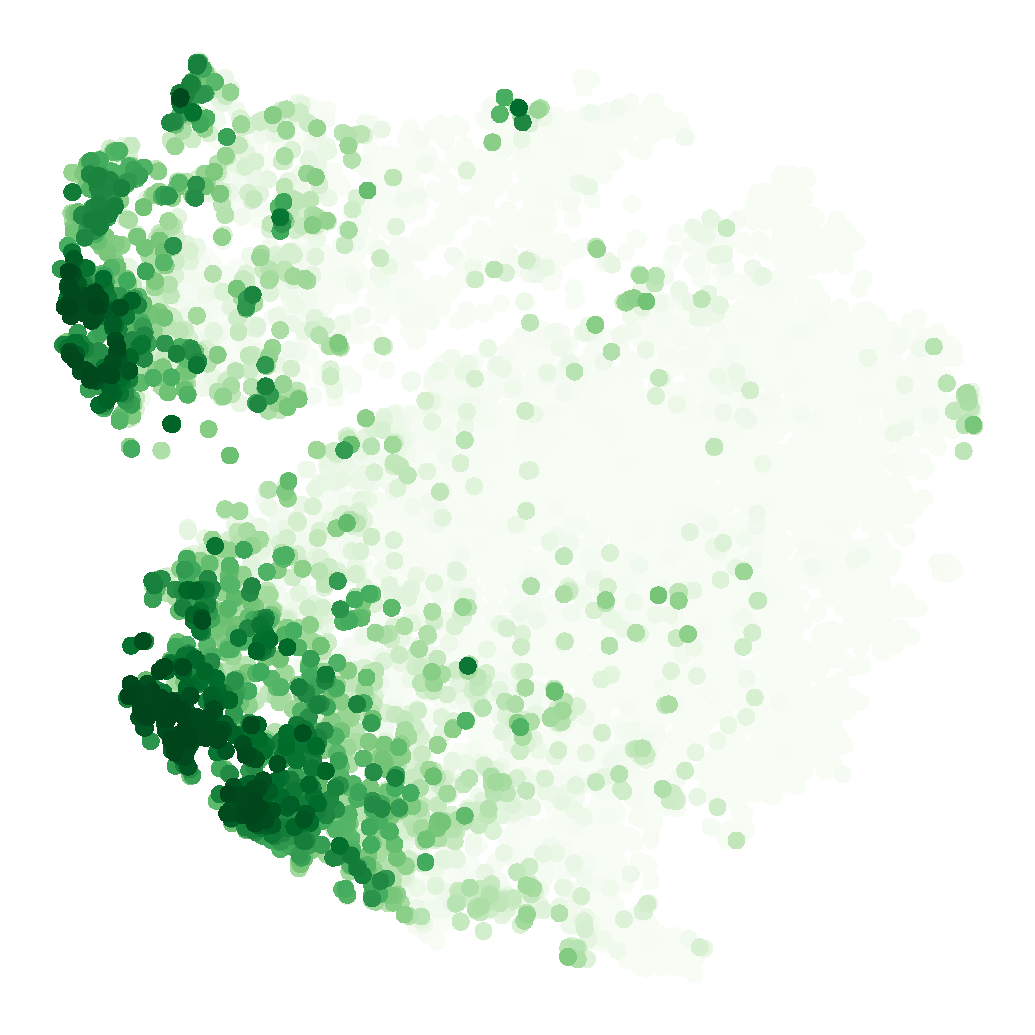
\includegraphics[width=\linewidth]{figures/appendix/tsne_probability_nocolorbar_perinuclear}
		\subcaption{Perinuclear}
		\vfill
		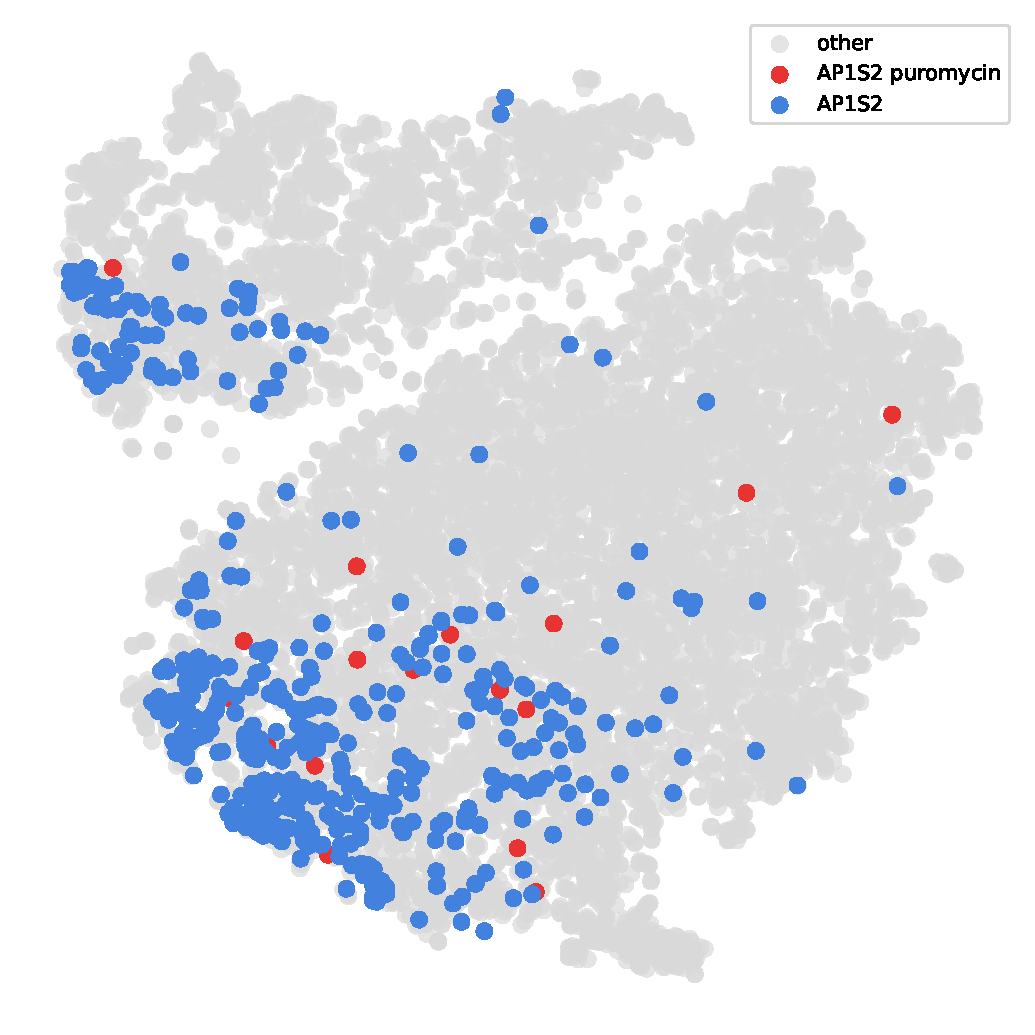
\includegraphics[width=\linewidth]{figures/appendix/tsne_perinuclear_AP1S2}
		\subcaption{AP1S2}
	\endminipage\hfill
	\minipage{0.2\textwidth}
		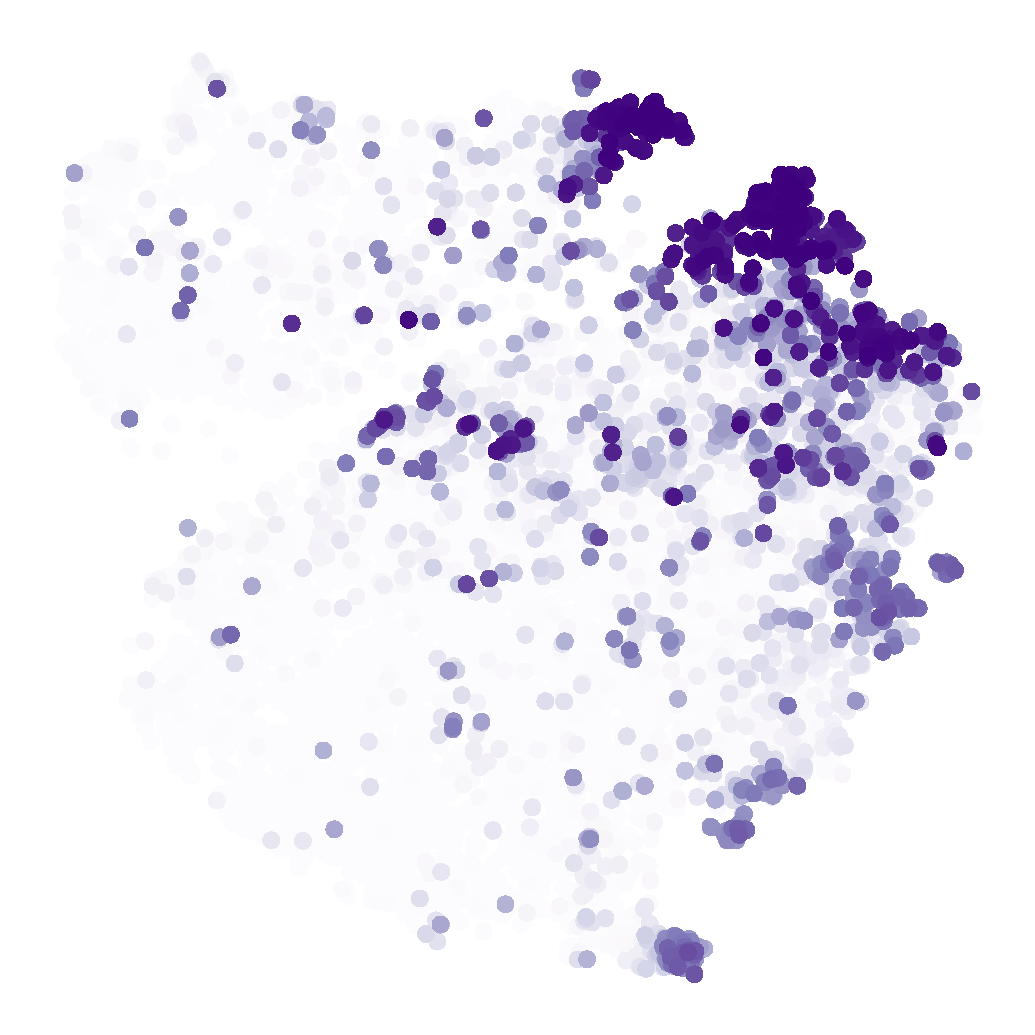
\includegraphics[width=\linewidth]{figures/appendix/tsne_probability_nocolorbar_protrusion}
		\subcaption{Protrusion}
		\vfill
		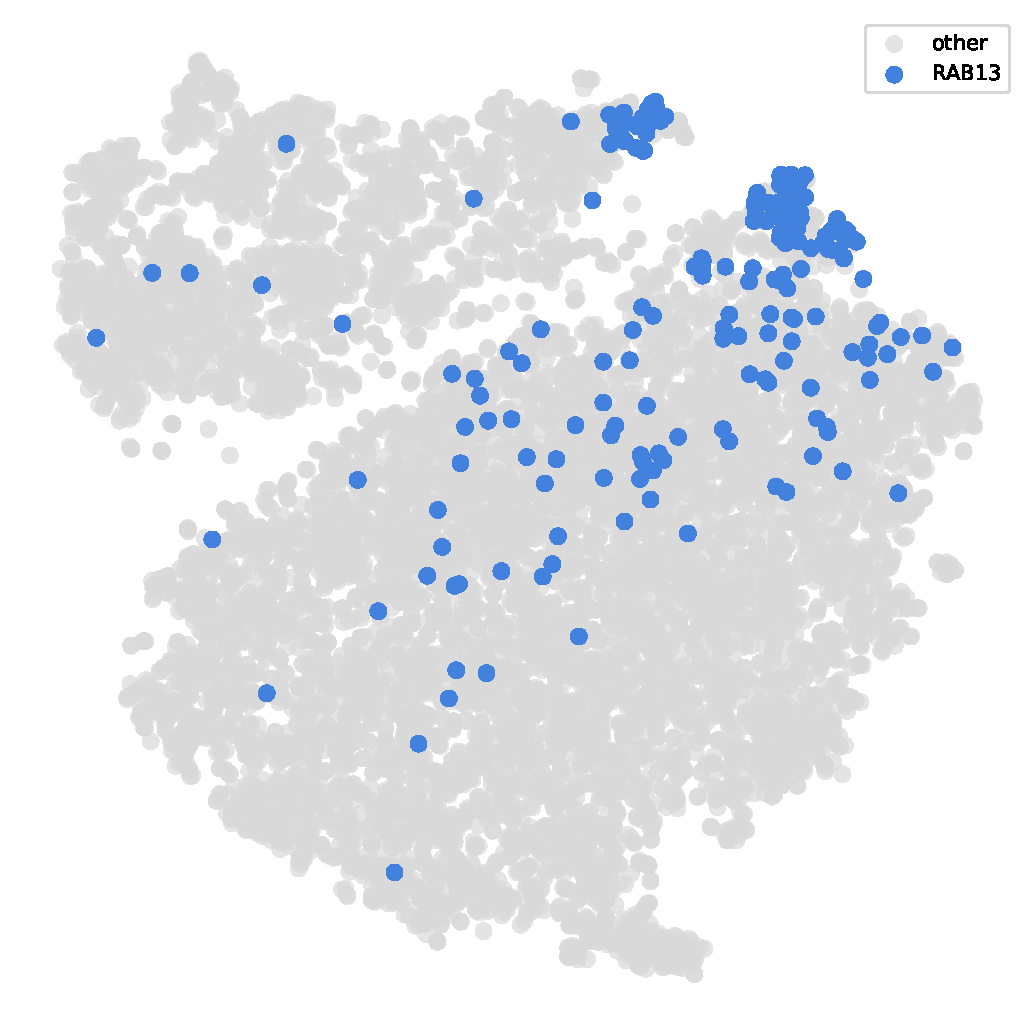
\includegraphics[width=\linewidth]{figures/appendix/tsne_protrusion_RAB13}
		\subcaption{RAB13}
	\endminipage
	\caption[Cell-wise results of localization pattern classification]{(\textit{Top}) Visualization of random forest classification probabilities in the t-SNE, from~\cite{CHOUAIB_2020}.
	Color indicates the probabilities of the cell to be classified in the indicated localization pattern.
	The darker, the higher the probability is.
	(\textit{Bottom}) Visualization of cells for some specific genes with the indicated localization pattern above.
	Cells can be untreated (\textit{blue}) or treated with puromycin (\textit{red})}
	\label{fig:tsne_proba_gene}
\end{figure}

On the bottom row we can observed how the cells for 5 different genes localize in the \ac{t-SNE} plot.
From the results presented in Figure~\ref{fig:heatmap_racha}, we also identify dominant localization patterns for these transcripts:
\begin{itemize}
	\setlength\itemsep{0.1em}
	\item DYNC1H1 with a foci and perinuclear patterns.
	\item CEP192 with an intranuclear pattern.
	\item SPEN with a nuclear edge pattern.
	\item AP1S2 with a perinuclear and a small foci patterns.
	\item RAB13 with a protrusion and a small foci patterns.
\end{itemize}

\noindent
These localizations observed at the gene level are consistent with the manual annotations in Figure~\ref{fig:tsne_annotation_racha} and \ac{t-SNE} regions interpreted from the top row of Figure~\ref{fig:tsne_proba_gene}.

A last observation that can be made from Figure~\ref{fig:tsne_proba_gene} is the apparent diversity of patterns observed at the gene level.
For example, cells where we spot DYNC1H1 transcripts are polarized toward the nucleus-related regions of the point cloud.
Moreover, a majority of untreated cells are in the foci-related region, while those treated with puromycin present a more uniform distribution across the \ac{t-SNE}.
Such results are consistent with the observed impact of the puromycin for genes like DYNC1H1 presenting a transcription factory pattern.

\section{Cell-wise pattern heterogeneity}
\label{sec:pattern_heterogeneity}

Another way to visualize the heterogeneity in terms of localization patterns is to plot the predicted probabilities for every cell in a heat map.
In Figure~\ref{fig:heatmap_racha_cells}, I adapt the results aggregated by genes from Figure~\ref{fig:heatmap_racha}.
It clearly appears that, for a given gene, the observed localization patterns are noisy.
Even if SPEN transcripts localize most of the time along the nucleus membrane, they also can be observed forming a cluster of \ac{RNA}s.
For some cells we do not even observe a specific pattern.
Such heterogeneity justifies the use of a quantitative pipeline to produce statistical results over a large population of cells.

These heat maps also confirm that different localization patterns can coexist for the same transcript but not necessarily within the same cells at the same time.
For example with ASPM transcripts, cells are identified with a foci pattern, a nuclear edge pattern or both at the same time.

\begin{figure}[h]
    \centering
    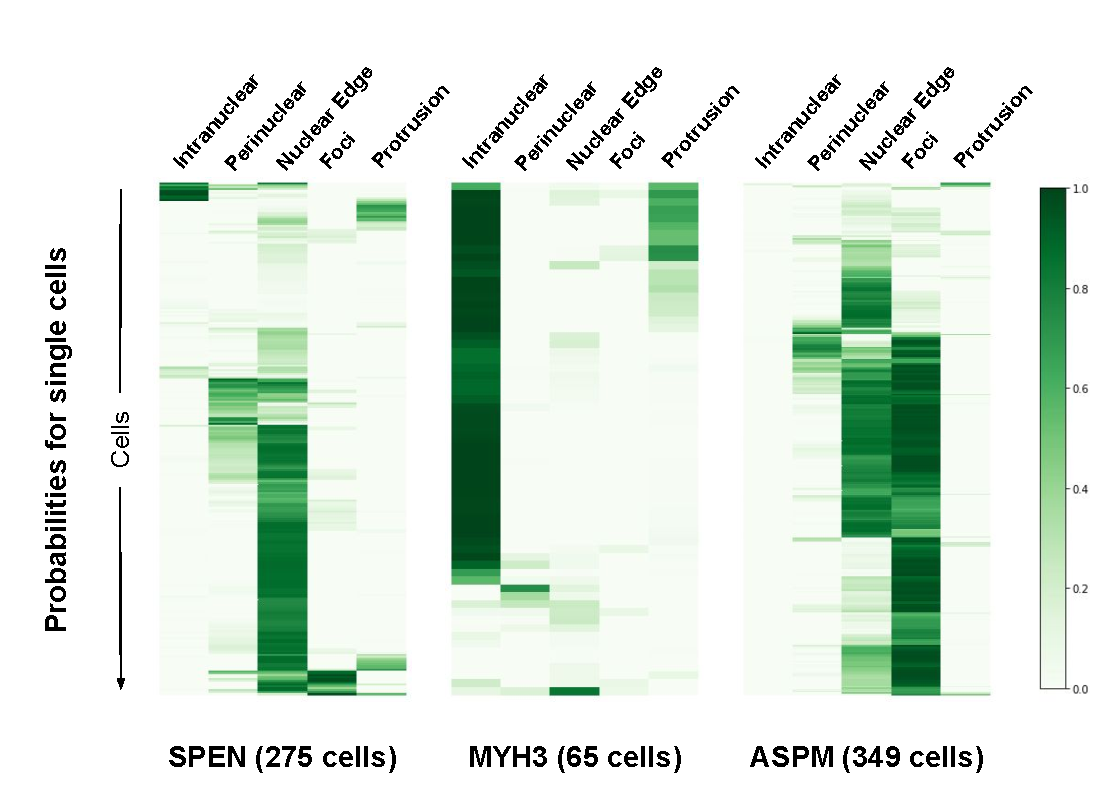
\includegraphics[width=\textwidth]{figures/appendix/heatmap_cell_racha}
    \caption[Heat maps with cell-wise classification results]{Three heat maps from~\cite{CHOUAIB_2020} with the probability of single cells to have each patterns.
	Only cells where we visualized SPEN, MYH3 and ASPM transcripts are represented.
	Each row corresponds to a cell and the color indicates the probabilities of the cell to be classified in the indicated localization pattern}
    \label{fig:heatmap_racha_cells}
\end{figure}
